\documentclass[a4paper,12pt]{article} % добавить leqno в [] для нумерации слева
\usepackage[a4paper,top=1.3cm,bottom=2cm,left=1.5cm,right=1.5cm,marginparwidth=0.75cm]{geometry}
%%% Работа с русским языком
\usepackage{cmap}					% поиск в PDF
\usepackage{mathtext} 				% русские буквы в фомулах
\usepackage[T2A]{fontenc}			% кодировка
\usepackage[utf8]{inputenc}			% кодировка исходного текста
\usepackage[english,russian]{babel}	% локализация и переносы

\usepackage{multirow}
\usepackage{graphicx}
\usepackage{mathtools}
\usepackage{wrapfig}
\usepackage{tabularx}
\usepackage{amssymb}
\usepackage{hyperref}
\usepackage[rgb]{xcolor}
\hypersetup{colorlinks=true,urlcolor=blue}
%% Шрифты
\usepackage{euscript}	 % Шрифт Евклид
\usepackage{amsmath}
\usepackage{mathtools}
%%% Заголовок
\author{Lokhmatov Arseniy}
\title{Лабораторная работа по общей физике}

\date{\today}
\begin{document}
\begin{titlepage}
    \newpage
    \begin{center}
    {\large МОСКОВСКИЙ ФИЗИКО-ТЕХНИЧЕСКИЙ ИНСТИТУТ (НАЦИОНАЛЬНЫЙ ИССЛЕДОВАТЕЛЬСКИЙ УНИВЕРСИТЕТ)}
    \vspace{1cm}

    {\largeФизтех-школа аэрокосмических технологий}
    \vspace{6em}
    \end{center}
    
    \vspace{1.2em}

    \begin{center}
    %\textsc{\textbf{}}
    \Large Лабораторная работа №4.7.3 \\
    Излучение поляризованного света
    \linebreak
    \end{center}
    
    \vspace{11em}
    
    \begin{flushright}
                       {\large Работу выполнил\\
                       Лохматов Арсений Игоревич\\
                       Б03-303 }
    \end{flushright}

    \vspace{\fill}

    \begin{center}
        
\includegraphics[width=0.2\linewidth]{dasr.png}
    \end{center}

    \begin{center}
    Долгопрудный, 2025
    \end{center}

    \end{titlepage}

\section{Теоретическая часть}

\paragraph{Цель работы:} ознакомиться с методами получения и анализа поляризованного света.

\paragraph{Оборудование:} оптическая скамья с осветителем; зелёный светофильтр; два поляроида; чёрное ззеркало; поляризованная эбонитовая пластинка; стопа стеклянных пластинок; слюдяные пластинки разной толщины; пластинки в $1/4$ и $1/2$ длины волны; пластинки в одну длину волны для зелёного света (пластинка чувствительного оттенка).

\paragraph{Определение направления разрешённой плоскости колебаний поляроида.} Определить направление разрешённых колебаний поляроида возможно с помощью чёрного зеркала.

При падении света на отражающую поверхночть под углом Брюстера, свет в отражающем луче почти полностью поляризован, а веркот $\mathbf{E}$ параллелен отражающей поверхночти. Луч света, прошедший поляроид и отразившийся от чёрного зеркала, имеет минимальную интенсивность при выполнении двух условий: во-первых свет падает на отражающую поверхность под углом Брюстера и, во вторых, в падающем пучке вектор $\textbf{E}$ лежит в плоскости падения.

Вращая поляроид вокруг направдения луча и чёрное ззеркало вокруг оси, перпендикулярной лучу, методом последовательных приближений можно добиться минимальной яркости луча, отражённого от зеркала, и таким образом определить разрешённое направление поляроида.

Изменяя угол поворота зеркала (угол Брюстера), нетрудно определить коэффициент преломления материала, из которого изготовлено зеркало. 

\paragraph{Получение эллиптически поляризованного света.}

\begin{wrapfigure}{r}{0.35\linewidth} 
    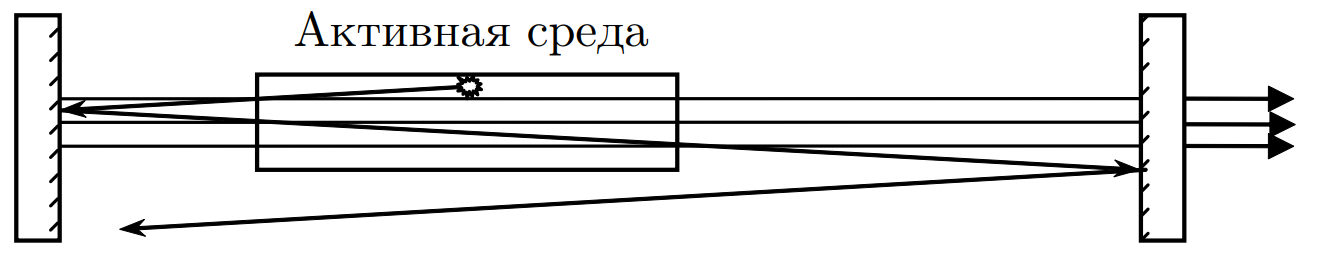
\includegraphics[width=\linewidth]{image1.png}
    \caption{Разложение линейно поляризованного света по главным направлениям двоякопреломляющей пластинки}
    \label{img1}
\end{wrapfigure}

Эллиптически поляризованный свет можно получить из линейно поляризованного с
помощью двоякопреломляющих кристаллических пластинок.

Двоякопреломляющая пластинка имеет два взаимно перпендикулярных главных направления, совпадающих с осями эллипсоида диэлектрической проницаемости. Волны, поляризованные вдоль главных направлений, распространяются в пластинке с разными скоростями, не изменяя характера своей поляризации. Эти волны называются главными. Мы будем обозначать показатели преломления для главных волн через $n_x$ и $n_y$, где $x$ и $y$ --- главные направления кристаллической пластинки (рисунок $\ref{img1}$).

Пусть на пластинку падает линейно поляризованная волна, электрический вектор которой ориентирован под некоторым углом $\alpha$ к оси
$x$. Разложим вектор $\mathbf{E}$ на составляющие $E_x$ и $E_y$. На входе пластинки $E_x$ и $E_y$ находятся в фазе. На выходе из-за разности скоростей между ними появляется разность хода $d(n_x-n_y)$, при этом сдвиг фаз определяется соотношением

\[ \Delta \phi =  \dfrac{2\pi}{m} = k d(n_x - n_y) \]

Как уже отмечалось, при сложении двух взаимно перпендикулярных колебаний, обладающих некоторым сдвигом фаз, образуется колебание, поляризованное по эллипсу.

Рассмотрим практически важные частные случаи.

\begin{wrapfigure}{l}{0.35\linewidth}
    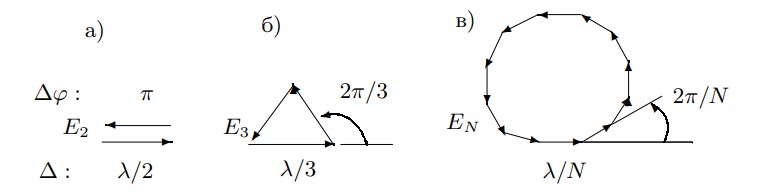
\includegraphics[width=\linewidth]{image2.png}
    \caption{Поворот направления колебаний с помощью пластинки в $\lambda/2$}
    \label{img2}
\end{wrapfigure}

 \begin{enumerate}
 		
 	\item Пластинка даёт сдвиг фаз $ 2\pi $ (пластинка в длину волны $ \lambda $). В результате сложения волн на выходе пластинки образуется линейно поляризованная волна с тем же направлением колебаний, что и в падающей волне.

	\item Пластинка даёт сдвиг фаз $\pi$ (пластинка в полдлины волны $\lambda/2$). На выходе пластинки снова образуется линейно поляризованная волна. Направление $bb'$ колебаний этой волны повёрнуто относительно направления $aa'$ колебаний падающей волны (рисунок $\ref{img2}$). Как нетрудно сообразить, направление $bb'$ является зеркальным отображением направления $aa'$ относительно одного из главных направлений пластинки. Такую пластинку используют для поворота направления колебаний линейно поляризованного света.
	
	\item Пластинка создаёт между колебаниями сдвиг фаз $\pi/2$ (пластинка в четверть длины волны). При сложении двух взаимно перпендикулярных колебаний, имеющих разность фаз $\pi/2$, образуется эллипс, главные оси которого совпадают с координатными осями $x$ и $y$. При равенстве амплитуд возникает круговая поляризация.
 	
 \end{enumerate}

Следует отметить, что, говоря о пластинках $\lambda,\text{ } \lambda/2,\text{ } \lambda/4$ и т. д., всегда подразумевают какую-либо вполне определённую монохроматическую компоненту (например, пластинка $\lambda/2$ для зелёного света). Если на двоякопреломляющую пластинку падает не монохроматический свет, то на выходе из неё для разных спектральных компонент эллипсы поляризации будут различными.

\paragraph{Анализ эллиптически поляризованного света.} Анализ эллиптически поляризованного света сводится к нахождению главных осей эллипса поляризации и к определению направления вращения электрического вектора.

Главные оси эллипса поляризации определяются с помощью анализатора по максимуму и минимуму интенсивности проходящего света. Направление вращения электрического вектора может быть найдено с помощью пластинки в четверть длины волны, для которой известно, какая из главных волн, $ E_x $ или $ E_y $, имеет б\'{o}льшую скорость распространения (и соответственно меньшее значение показателя преломления).

Выберем для определённости координатные оси $x$ и $y$ на пластинке так, чтобы $nx<ny$. В этом случае главная волна $E_x$ имеет большую скорость распространения. Поместим такую пластинку на пути эллиптически поляризованного света и совместим главные направления пластинки $\lambda/4$ с главными осями эллипса поляризации. На выходе из этой пластинки сдвиг фаз между $E_x$ и $E_y$ вместо $\pi/2$ станет равным нулю или $\pi$. Свет окажется линейно поляризованным. Из двух возможных значений сдвига фаз, $0$ или $\pi$, реализуется только то, которое соответствует имеющемуся в волне направлению вращения электрического вектора.

Рассмотрим, например, случай, когда электрический вектор в эллиптически поляризованной волне вращается против часовой стрелки, если смотреть навстречу лучу. В этом случае, очевидно, в волне, падающей на пластинку в $\lambda/4$, колебание $E_y$ отстаёт по фазе на $\pi/2$ от колебания $E_x$. При прохождении через пластинку разность фаз увеличивается до $\pi$. Таким образом на выходе из пластинки возникают линейно поляризованные волны со сдвигом фаз $\pi$. Сложение этих волн даёт плоскополяризованную волну, электрический вектор которой располагается во втором и четвёртом квадрантах координатной системы $x,\text{ }y$.

Рассуждая аналогичным образом, найдём, что при вращении электрического вектора по часовой стрелке направление колебаний в линейно поляризованной волне, выходящей из пластинки, располагается в первом и третьем квадрантах. Определяя направление колебаний на выходе из пластинки с помощью поляроида, можно, таким образом, определить характер эллиптической поляризации (вращение против или по часовой стрелке).

\paragraph{Пластинка чувствительного оттенка.}

\begin{wrapfigure}{l}{0.35\linewidth}
    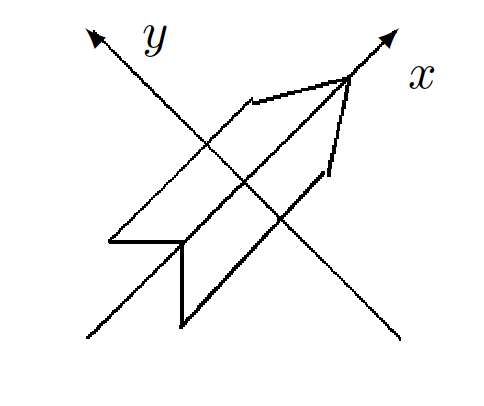
\includegraphics[width=\linewidth]{image3.png}
    \caption{Пластинка чувствительного оттенка}
    \label{img3}
\end{wrapfigure}

Выше предполагалось известным, какому из двух главных направлений пластинки в четверть длины волны соответствует большая скорость распространения света. Установить это можно различными способами, например с помощью пластинки чувствительного оттенка (так называют пластинку в $\lambda$ для зелёной спектральной компоненты, $\lambda=560$ нм).

Пластинка имеет форму стрелы (рисунок $\ref{img3}$), вдоль оси которой расположено главное направление, соответствующее большей скорости распространения.

Если пластинка чувствительного оттенка помещена между скрещенными поляроидами и главные направления пластинки не параллельны направлениям разрешённых колебаний поляроидов, то при освещении
белым светом пластинка кажется окрашенной в лилово-красный цвет. Это объясняется тем, что зелёная компонента линейно поляризованного света при прохождении пластинки не меняет поляризации и задерживается вторым поляроидом. Для красной и фиолетовой компонент пластинка создаёт сдвиг фаз, несколько отличный от $2\pi$. На выходе из пластинки красная и фиолетовая компоненты оказываются поэтому эллиптически поляризованными и частично проходят через второй поляроид. Таким образом, в известном смысле наблюдаемый в указанном опыте цвет пластинки дополнителен к зелёному.

Если между скрещенными поляроидами поместить пластинку чувствительного оттенка ($\lambda$) и пластинку в $\lambda/4$ так, чтобы их главные направления совпадали, цвет пластинки изменится. Если у пластинки чувствительного оттенка и пластинки в $\lambda/4$ совпадут главные направления, соответствующие большей скорости распространения, то разность хода между $E_x$ и $E_y$ для зелёного света составит уже $5\lambda/4$. Это соответствует разности хода в $\lambda$ для света с большей длиной волны, т. е. для "<более красного"> света. При освещении этих пластинок (напомним, что они расположены между скрещенными поляроидами) белым светом теперь погасится не зелёная, а красная часть спектра, и проходящий свет будет казаться зеленовато-голубым. Если же главные направления, соответствующие большей скорости распространения, у пластинки чувствительного оттенка и у пластинки в $\lambda/4$ окажутся перпендикулярными, то проходящий свет приобретёт оранжево-желтую окраску (погасится фиолетово-голубая часть спектра).

Изменение цвета позволяет, таким образом, определить, какое из главных направлений пластинки в $\lambda/4$ соответствует большей скорости распространения.

\paragraph{Интерференция поляризованных лучей}

\begin{wrapfigure}{r}{0.35\linewidth}
    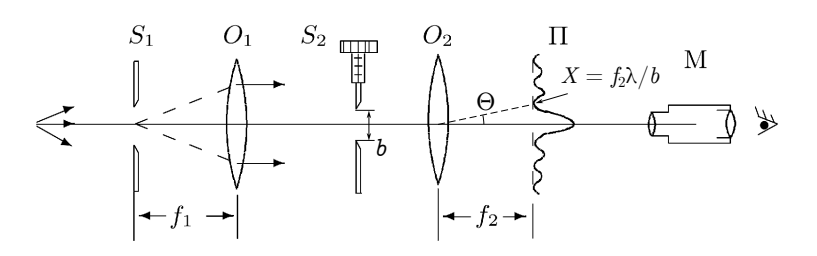
\includegraphics[width=\linewidth]{image4.png}
    \caption{К объяснению интерференции поляризованных лучей}
    \label{img4}
\end{wrapfigure}


Тонкие двоякопреломляющие пластинки, помещённые между поляроидами, кажутся окрашенными. Эта окраска может быть истолкована как результат интерференции поляризованных лучей. На рисунке $\ref{img4}$ представлена схема для случая скрещенных поляроидов.

Здесь $p_1p'_1$ --- разрешённое направление колебаний поляризатора (первого поляроида); $x,\text{ }y$ --- координатная система, связанная с главными направлениями двоякопреломляющей пластинки; $p_2p'_2$ --- разрешённое направление колебаний анализатора (второго поляроида). Волны $E_x$ и $E_y$ на выходе из пластинки когерентны, но не могут интерферировать, так как $E_x\perp E_y$. Волны $E_1$ и $E_2$ на выходе второго поляроида также являются когерентными и к тому же поляризованы в одной плоскости. Эти волны интерферируют между собой. Результат интерференции определяется зависящим от длины волны сдвигом фаз между $E_1$ и $E_2$. В результате интерференции поляризованных лучей пластинка, освещаемая белым светом, кажется окрашенной.

Если поворачивать двоякопреломляющую пластинку, расположенную между скрещенными поляроидами, то соотношение амплитуд волн $E_1$ и $E_2$ и разность фаз между ними не изменяются. Это означает, что цвет пластинки при её поворотах не меняется, а меняется только интенсивность света. За один оборот пластинки интенсивность четыре раза обращается в нуль --- это происходит при совпадении главных направлений $x$ и $y$ с разрешёнными направлениями колебаний поляроидов.

Если же двоякопреломляющую пластинку оставить неподвижной, а второй поляроид повернуть так, чтобы разрешённые направления $p_1p'_1$ и $p_2p'_2$ совпали, то волны $E_1$ и $E_2$ приобретают дополнительный фазовый сдвиг на $\pi$ для всех спектральных компонент; при этом их амплитуды изменятся так, что цвет пластинки изменится на дополнительный.

\section{Практическая часть}

\begin{wrapfigure}{r}{0.35\linewidth}
    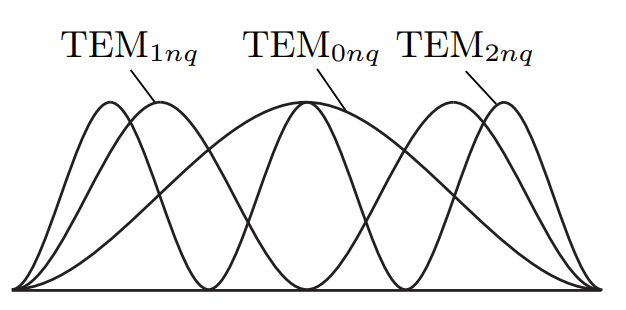
\includegraphics[width=\linewidth]{image5.png}
    \caption{Определение разрешённого направления поляроида}
    \label{img5}
\end{wrapfigure}

В работе предлагается с помощью чёрного зеркала определить разрешнные направления поляроидов; определить характер поляризации света, прошедшего стопу  и отражённого от неё под углом Брюстера; оценить угол Брюстера для эбонита; выделить пластинки $\lambda/2$ и $\lambda/4$; определить направление большей и меньшей скоростей для пластинки $\lambda/4$; исследовать интерференцию поляризованных лучей.

\subsection{Определение разрешённых направлений поляроида}

\begin{enumerate}
    \item Разместили на оптической скамье осветитель $S$, поляроид $P_1$ и чёрное зеркало (рисунок $\ref{img5}$);

    \item поворачивая поляроид вокруг направления луча, а чёрное зеркало вокруг вертикалной оси, методом последовательных приближений добились наименьшей яркости отражённого пятна. Определили разрешённое направление поляроида, $\varphi=(313\pm1)$ градус.

    \item Поставили вместо зеркала второй поляроид и определили его разрешённое направление, скрестив поляроиды, $\varphi=(55\pm1)$ градус. В итоге, первый поляроид усовно пропускает $s-$поляризованную волну, а второй поляроид - $p-$поляризованную.
\end{enumerate}

\subsection{Определение угла Брюстера для эбонита}

\begin{enumerate}
    \item Поставили на скамью вместо чёрного зеркала (рисунок $\ref{img5}$) эбонитовую пластину и определили по лимбу угол Брюстера для эбонита. Получили, что $\varphi_{\text{Бр}}=(307\pm1)$ градус. Неточность установки угла, помимо неточности человеческого глаза, вносит приборная погрешность лимба, а так же тот факт, что в этом случае на эбонитовую пластину падают лучи всех цветовых компонент.

    \[ \varphi_{\text{Бр}}=\arctan{n} \Longleftrightarrow n=\tan{\varphi_{\text{Бр}}} \Longrightarrow \]
    \[ \Longrightarrow n=\tan{\Big((360-307)\cdot\frac{\pi}{180}\Big)} = (1.33\pm0.02)\text{, }\varepsilon=1.5\% \]

    \item Повторили измерения, добавив светофильтр $\text{Ф}$, $\varphi_{\text{Бр}}=(302\pm1)$ градус. В этом случае мы точнее определили угол полного внутреннего отражения, поскольку светофильтр пропускает конкретную длину волн.

    \[ \varphi_{\text{Бр}}=\arctan{n} \Longleftrightarrow n=\tan{\varphi_{\text{Бр}}} \Longrightarrow \]
    \[ \Longrightarrow n=\tan{\Big((360-302)\cdot\frac{\pi}{180}\Big)} = (1.60\pm0.02)\text{ рад, }\varepsilon=1.25\% \]

    \item Табличный результат составляет $n^{tab}_{\text{эбонит}}=1.37$. Видим, что полученные нами результаты совпадают по порядку величины и довольно близки к табличному.
\end{enumerate}

\subsection{Исследование стопы}

Поставили вместо эбонитового зеркала $\ref{img5}$ стопу стеклянных пластинок и подобрали для неё такое положение, при котором свет падает на неё под углом Брюстера.

\begin{wrapfigure}{r}{0.35\linewidth}
    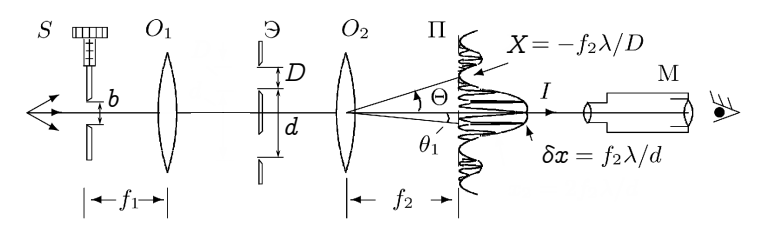
\includegraphics[width=\linewidth]{image6.png}
    \caption{Исследование стопы}
    \label{img6}
\end{wrapfigure}

Осветили стопу неполяризованным светом и, рассматривая через поляроиды (рисунок $\ref{img6}$) отражённый от стопы и преломлённый лучи, определили в них ориентацию веткора $\mathbf{E}$.

Посмотрели через поляроид $P_1$ на преломлённый луч, мы его чётко увидели. Затем посмотрели на отражённый луч, его увидели намного тусклее. После этого сменили поляроид на $P_2$, в этом случае ситуация сменилась на противоположную -- отражённый луч мы видели хорошо, а вот преломлённый практически не видели. 

Поскольку эти поляроиды скрещены, то в идеале мы не должны были видеть отражённый луч через поляроид $P_1$ и преломлённый луч через поляроид $P_2$. Но из наших наблюдений можно сделать вывод, что стопа частично поляризует свет.

\subsection{Определение главных плоскостей двоякопреломляющих пластин}

Поставили однородную кристаллическую пластинку между скрещёнными поляроидами $P_1$ и $P_2$ (рисунок $\ref{img7}$).

\begin{wrapfigure}{r}{0.35\linewidth}
    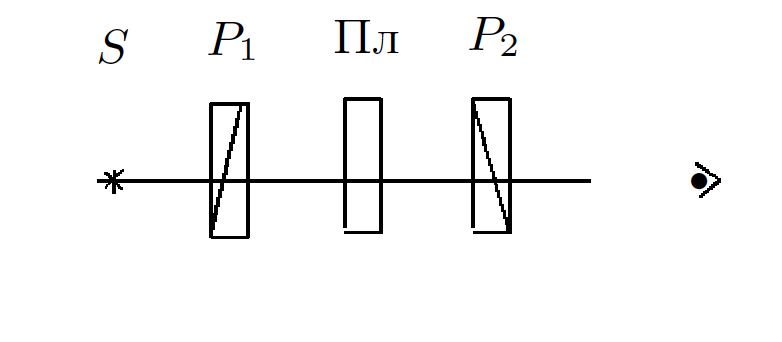
\includegraphics[width=\linewidth]{image7.png}
    \caption{Определение главных направлений в пластинках}
    \label{img7}
\end{wrapfigure}

Вращая пластинку вокруг направления луча и наблюдая за интенсивностью света, проходящего сквозь второй поляроид, определили, что главные направления пластинки совпадают с разрешёнными направлениями поляроидов при условии, что вектор $\mathbf{E}$ спроецирован на быстрые и медленные направления за счёт поворота поляроида на угол порядка $\approx45$ градусов относительно минимума.

Повторили опыт для второй пластинки, результат аналогичный.

\subsection{Выделение пластин $\lambda/2$ и $\lambda/4$}

Добавили к схеме, изображённой на рисунке $\ref{img7}$, зелёный светофильтр; установили разрешённое направление поляроида горизонтально, а главные главные направления исследуемой пластинки -- под углом $45$ градусов к горизонтали.

Смотря через поляроид $P_2$ на пластинку, вращаем поляроид. Если интенсивность лучей не падает, то это означает, что свет имеет круговую поляризацию на выходе из пластинки. В этом случае мы можем наблюдать, что цвет лучей изменяется. Это можно аргументировать тем, что мы изменяет разрешённое направление поляроида для тех или иных цветов. Но интенсивность не изменяется! Значит это пластинка $\lambda/4$, которая изменяет фазовую характеристику волны на $\pi/2$.

Если же интенсивность лучей падает при вращении поляроида, мы можем различить минимум и максимум, то это означает, что свет на выходе из пластинки поляризован линейно. Значит это пластинка $\lambda/2$, которая изменяет фазовую характеристику волны на $\pi$.

\subsection{Определение направления большей и меньшей скорости в пластинке $\lambda/4$}

\begin{wrapfigure}{r}{0.35\linewidth}
    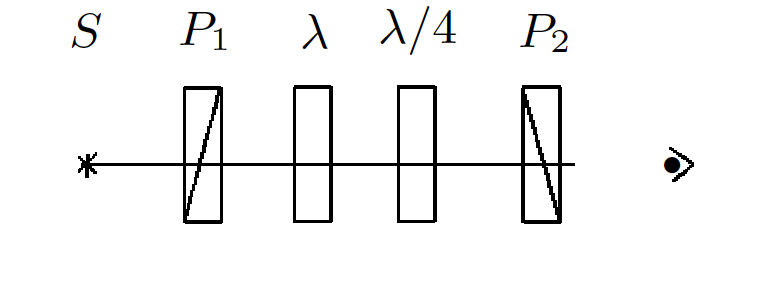
\includegraphics[width=\linewidth]{image8.png}
    \caption{Определение направлений большей и меньшей скоростей}
    \label{img8}
\end{wrapfigure}

\begin{enumerate}
    \item Поставили между скрещёнными поляроидами пластинку чувствительного оттенка ($\lambda$ для зелёного света), имеющую вид стрелки. Световой вектор, оринентированный вдоль направления стрелки, проходит с большей скоростью, перпендикулярный -- с меньшей.
    Установили разрешённое направление первого поляроида горизонтально, второй поляроид скрестили с первым. Поставили между ними фильтр и пластинку чувствительного оттенка, наблюдаем минимум через второй поляроид. Когда мы убираем пластинку, минимум сохранялся, а это значит, что эта пластинка не меняет поляризацию зелёного света в условиях предыдущего опыта.
    \item Убрали зелёный фильтр и поставили между скрещёнными поляроидами пластинку $\lambda$. Глядя сквозь второй поляроид на стрелку, убедились, что она имеет пурпурный цвет. Это происходит из-за того, что зелёный свет задерживается вторым поляроидом (изначально поляроиды были скрещены для длины волны зелёного света), а красная и синяя компоненты проходят.
    \item Добавили к схеме пластинку $\lambda/4$ (рисунок $\ref{img8}$), главные направления которой совпадают с главными направлениями пластины $\lambda$ и ориентированы под углом $45$ градусов к разрешённым направлениям скрещённых поляроидов.
    При повороте рейтера со стрелкой на $180$ градусов вокруг вертикальной оси цвет стрелки меняется от зелёно-голубого до оранжево-жёлтого. Дело в том, что в зависимости от того, совпадают или не совпадают быстрые оси поляроидов, совокупность пластинок даёт либо $3\pi/4$, либо $5\pi/4$, что соответствует жёлтому и синему цветовым оттенкам. 
\end{enumerate}

\subsection{Интерференция поляризованных лучей}

Расположили между скрещёнными поляроидами мозаичную слюдяную пластинку. Главные направления всех пластинок ориентированы параллельно сторонам квадрата.

Вращая пластинку, наблюдаем за изменениями цвета или интенсивности в отдельных квадратиках. Теперь, не трогая пластинки, вращаем второй поляроид -- цвета так же меняются. 

В первом случае, разные квадратики пластинки имеют разную "толщину", и при повороте пластинки проходящий свет через пластинку поляризуется по разному, в результате чего цве или интенсивность меняются в отдельных квадратиках. 

Во втором случае, вращая поляроид, мы изменяем тип поляризации, в результате чего свет на выходе из пластинки поляризуется по разному, происходит так же смена цвета. Допустим, может сложиться ситуация, что пластинка и второй поляроид скрещены для определённого типа цвета, поэтому он не проходит.

\subsection{Определение направления вращения светового вектора в эллиптически поляризованной волне}

\begin{enumerate}
    \item Нарисуем вектор поляризации для ветора $\mathbf{E}$, вышедшего из пластинки $\lambda/4$, и укажем на нём направления большей и меньшей скорости. Рядом нарисуем две вышедших из пластинки синусоиды: $x(t)$ и $y(t)$ со сдвигом фаз в четверть периода. Результат представлен на рисунке $\ref{img9}$.

    \item Снова поставили зелёный фильтр, а за ним между скрещёнными поляроидами -- пластинку произвольной толщины, например, $\lambda/4$. 

    \item Получили эллиптически поляризованный свет. Для этого установили разрешённое направление первого поляроида под углом $10-20$ градусов к горизонтали так, чтобы вектор $\mathbf{E}$ падающего на пластинку света был расположен в первом квадранте. Установили разрешённое направление второго поляроида вертикально и, вращая пластинку, нашли минимальную интенсивность света, прошедшего второй поляроид. Вращая второй поляроид убедились, что свет поляризован эллиптически.

    Таким образом, мы получили эллипс поляризации с вертикально ориентированной малой осью.

    \item Для определения направления вращения светового вектора в эллипсе установили между поляроидами дополнительную пластинку $\lambda/4$ с известными направлениями "быстрой" и "медленной" осей, ориентированными по осям эллипсапляризации анализируемого света. В этом случае вектор $\mathbf{E}$ на выходе будет таким, как если бы свет прошёл две пластинки $\lambda/4$: в совокупности они дают пластинку $\lambda/2$ или $0\cdot\lambda$, которая линейно поляризует свет.

    То есть, пластинки по одиночке дают эллипсы, вращающиеся в разные стороны, но поставленные друг за другом, они скомпенсируют разность фаз.
\end{enumerate}

\begin{figure}[h]
\begin{center}
    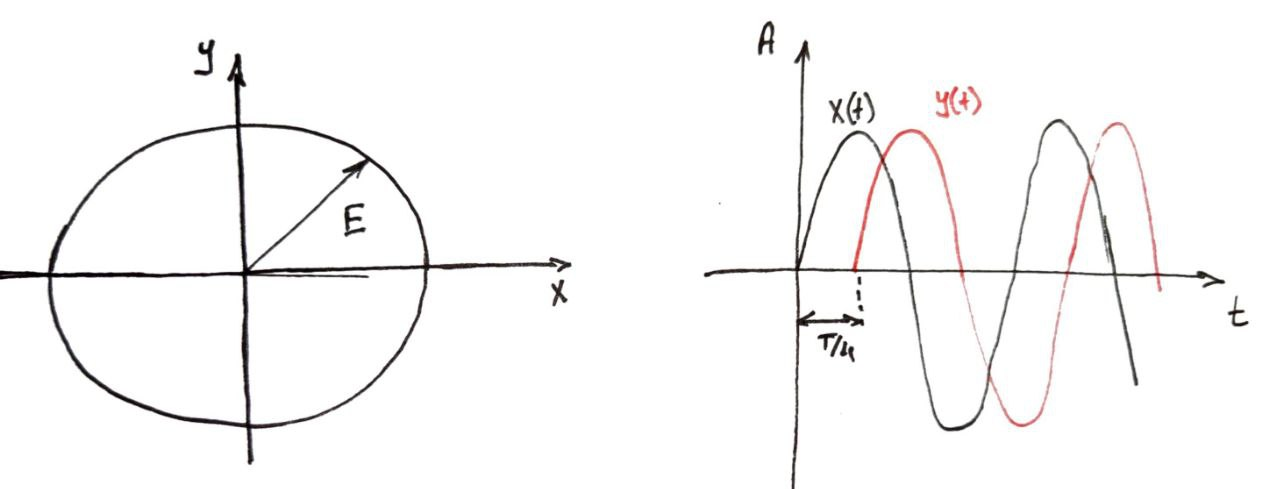
\includegraphics[width=16cm]{image9.jpg}
\end{center}
    \caption{Эллипс поляризациидля вектора $\mathbf{E}$, вышедшего из пластинки $\lambda/4$}
    \label{img9}
\end{figure}

\newpage

\section{Подведение итогов и выводы}

В данной лабораторной работе мы изучали поляризованный свет, поставили серию экспериментов, по результатам которых:
\begin{enumerate}
    \item определили разрешённые направления поляроидов,
    \item определили угол Брюстера для эбонита,
    \item исследовали стопу Столетова,
    \item определили главные плоскости двоякопреломляющих пластин,
    \item научились различать пластинки $\lambda/4$ и $\lambda/2$ как поляризоторы,
    \item определили напарвление большей и меньшей скорости в пластинке $\lambda/4$,
    \item исследовали интерференцию поляризованных лучей,
    \item исследовали направления вращения светового вектора в эллиптически поляризованной волне.
\end{enumerate}

Наблюдаемые явления полностью согласуются с теоретическими выкладками, что говорит о точности проведения данных экспериментов. 

\end{document}
